\documentclass[11pt]{article}
\usepackage[margin=0.85in]{geometry}
\usepackage[T1]{fontenc}
\usepackage{hyperref}
\usepackage{graphicx}
\usepackage{array}
\usepackage{longtable}

\title{Homework 5: Vision Transformers for Image Classification}
\author{Gilberto Feliu \\ Student ID: 801257813}
\date{July 20, 2026}

\begin{document}
\maketitle

\noindent\textbf{Assignment:} Homework 5 \\
\textbf{Course:} ECGR 4106 \\
\textbf{GitHub Repository:} \url{https://github.com/gfeliu-rgb/ECGR-4106-HW5}

\section*{Dataset and Experimental Setup}
Both problems use CIFAR-100 through \texttt{torchvision.datasets.CIFAR100}. Training images are normalized with CIFAR-100 channel statistics. Problem 1 uses 32 by 32 inputs with random crop, padding, and horizontal flip for training; evaluation uses only tensor conversion and normalization. Problem 2 uses 224 by 224 resized inputs for Swin-Tiny, Swin-Small, and the scratch Swin baseline.

The scripts select CUDA when available and otherwise run on CPU. The completed CSV summaries record CUDA for all Problem 1 runs and all Problem 2 runs. The final Problem 2 experiments were run with approved GPU access on an NVIDIA GeForce RTX 4070. Package versions used in the current environment were: \texttt{torch 2.12.0+cu130}, \texttt{torchvision 0.27.0+cu130}, \texttt{transformers 5.14.1}, \texttt{pandas 2.2.3}, \texttt{numpy 2.2.6}, and \texttt{matplotlib 3.10.9}.

Important status note: Problem 1 has 10-epoch results for all planned rows. Problem 2 has 5-epoch results for all planned rows. Every submitted summary row contains measured result values.

\section*{Grader Checklist and Artifact Map}
\begin{center}
\scriptsize
\begin{tabular}{|p{2.45in}|p{3.7in}|}
\hline
Requirement & Where it is shown \\
\hline
Full name, student ID, course, and assignment number & First page header of this report \\
\hline
Public GitHub repository & First page repository link and repository README \\
\hline
CIFAR-100 loaded with torchvision & Dataset section and both source scripts \\
\hline
Problem 1 ViT from scratch and ResNet-18 baseline & Problem 1 implementation summary, results table, and notebook \\
\hline
Problem 1 four ViT configurations & Problem 1 configuration table and Problem 1 summary CSV \\
\hline
Problem 1 parameters, FLOPs, runtime, and accuracy & Problem 1 results table, complexity section, and tradeoff figure \\
\hline
Problem 1 training behavior verification & Problem 1 training-curve figure and analysis paragraph \\
\hline
Problem 2 pretrained Swin-Tiny, Swin-Small, and scratch Swin & Problem 2 results table and \texttt{src/hw5\_swin.py} \\
\hline
Problem 2 model size and trainable parameter comparison & Problem 2 model-size section and tradeoff figure \\
\hline
Problem 2 training curves and discussion & Problem 2 training-curve figure and analysis paragraph \\
\hline
CPU fallback and executed notebooks & Device-selection code in both scripts; executed notebooks with visible outputs \\
\hline
\end{tabular}
\end{center}

The repository also includes the CSV files used to generate every table and plot. This is intended to make the final numbers traceable rather than only stated in the report.

\section*{Reproducibility and Metric Details}
CIFAR-100 contains 50,000 training images and 10,000 test images across 100 classes. The scripts train on the official training split and evaluate on the official test split. The CSV column names use \texttt{val\_loss} and \texttt{val\_accuracy\_pct}, but these values are computed on the CIFAR-100 test split because no separate validation split was created for this homework. Randomness is controlled with seed \texttt{4106} for Python and PyTorch.

All models use cross-entropy loss and top-1 accuracy. Training time is measured as average wall-clock seconds per epoch, including evaluation at the end of each epoch. The history CSV files in the two results folders contain the per-epoch losses, accuracies, and runtime values used for the plots. The main commands used to reproduce the artifacts are:

\begin{verbatim}
python src/hw5_vit_resnet.py --run-all-vit --run-resnet
python src/hw5_swin.py --run-pretrained swin_tiny_pretrained
python src/hw5_swin.py --run-pretrained swin_small_pretrained
python src/hw5_swin.py --run-scratch --epochs 5 --batch-size 32 \
  --image-size 224
python tools/make_hw5_plots.py
\end{verbatim}

\subsection*{Experimental Protocol Details}
The experiments were organized to make each comparison fair within the limits of the assignment. In Problem 1, every ViT configuration and the ResNet-18 baseline uses CIFAR-100, batch size 64, 10 epochs, Adam, and learning rate 0.001. This keeps the optimizer and schedule fixed so the main variables are architecture family, patch size, embedding dimension, depth, and attention-head count. I did not tune a separate learning rate for each architecture because that would make the comparison less direct.

In Problem 2, the pretrained Swin experiments follow the assigned transfer-learning setup: resize CIFAR-100 images to 224 by 224, replace the classifier head for 100 classes, freeze the backbone, and train only the head. The scratch Swin run uses the same 224 by 224 preprocessing so the comparison is not confounded by input resolution. The pretrained runs use the lower learning rate \texttt{2e-5}, while the scratch run uses \texttt{0.001}, matching the assignment instructions.

I treated the curves as a required part of the evaluation, not just a visual add-on. A final accuracy number can hide whether the model was learning steadily, saturating, overfitting, or staying at chance. For that reason, the report includes loss curves, accuracy curves, final tradeoff plots, and CSV history files so the grader can inspect the full training behavior behind each summary number.

\section*{Problem 1: Vision Transformer from Scratch vs. ResNet-18}
\subsection*{Objective}
The goal of Problem 1 is to compare several Vision Transformer configurations against a ResNet-18 baseline on CIFAR-100 and discuss accuracy, parameter count, estimated FLOPs, and training time.

\subsection*{Configurations}
\begin{center}
\scriptsize
\begin{tabular}{|p{0.85in}|r|r|r|r|r|r|r|r|}
\hline
Model & Patch & Embed & Depth & Heads & MLP & Epochs & Batch & LR \\
\hline
ViT-A & 4 & 256 & 4 & 4 & 1024 & 10 & 64 & 0.001 \\
\hline
ViT-B & 4 & 512 & 8 & 8 & 2048 & 10 & 64 & 0.001 \\
\hline
ViT-C & 8 & 256 & 4 & 4 & 1024 & 10 & 64 & 0.001 \\
\hline
ViT-D & 8 & 512 & 8 & 8 & 2048 & 10 & 64 & 0.001 \\
\hline
ResNet-18 & -- & -- & -- & -- & -- & 10 & 64 & 0.001 \\
\hline
\end{tabular}
\end{center}

\subsection*{Implementation Summary}
The custom ViT starts with a convolutional patch embedding layer whose kernel size and stride match the patch size. The flattened patch sequence is prepended with a learned class token, then combined with a learned positional embedding. The encoder is built from \texttt{nn.TransformerEncoderLayer} using GELU activations, multi-head self-attention, feed-forward MLP blocks, dropout, and layer normalization. The classifier uses the final normalized class-token representation and a linear head for 100 CIFAR-100 classes.

The ResNet-18 baseline uses \texttt{torchvision.models.resnet18(weights=None)}. Its first convolution is changed to a 3 by 3 stride-1 convolution and the initial max-pooling layer is removed so the model is better matched to 32 by 32 CIFAR images. All models use cross-entropy loss and Adam optimization. Evaluation runs without gradients on the CIFAR-100 test split and records validation/test loss and top-1 accuracy.

\subsection*{Complexity Calculation Details}
For each ViT, the number of tokens is $N = (32 / \mathrm{patch\_size})^2 + 1$, where the extra token is the class token. Patch embedding parameters are $(\mathrm{patch\_size}^2 \times 3 \times \mathrm{embed\_dim}) + \mathrm{embed\_dim}$. The learned class token and positional embedding add $\mathrm{embed\_dim} + N \times \mathrm{embed\_dim}$ parameters. Transformer and classifier parameters are counted directly from the PyTorch model.

ViT FLOPs are estimated per forward pass with the transformer approximation
$\mathrm{FLOPs}_{layer} \approx 4Nd^2 + 2N^2d + 2Ndm$, where $d$ is embedding dimension and $m$ is the MLP hidden dimension. The reported ViT FLOPs multiply that layer cost by the transformer depth and add the classifier head cost $d \times 100$. ResNet-18 FLOPs are estimated by summing convolution and linear multiply-adds from the actual CIFAR-adapted network, using the 3 by 3 stride-1 stem and removed max pool.

\subsection*{Results}
\begin{center}
\scriptsize
\begin{tabular}{|p{0.85in}|r|r|r|r|r|p{1.0in}|}
\hline
Model & Params & FLOPs & Time/Epoch & Val Loss & Test Acc. & Status \\
\hline
ViT-A & 3,214,692 & 2.13e8 & 23.01 & 3.2834 & 20.01\% & 10 epochs, CUDA \\
\hline
ViT-B & 25,330,276 & 1.67e9 & 106.72 & 4.3232 & 4.51\% & 10 epochs, CUDA \\
\hline
ViT-C & 3,239,268 & 5.41e7 & 12.22 & 3.8851 & 9.68\% & 10 epochs, CUDA \\
\hline
ViT-D & 25,379,428 & 4.30e8 & 42.30 & 4.2694 & 4.95\% & 10 epochs, CUDA \\
\hline
ResNet-18 & 11,220,132 & 5.55e8 & 61.24 & 1.3919 & 61.20\% & 10 epochs, CUDA \\
\hline
\end{tabular}
\end{center}

\subsection*{Analysis}
Among the ViT models, ViT-A performed best with 20.01\% test accuracy and a final validation loss of 3.2834. ViT-C was the next best ViT at 9.68\% while using the lowest estimated FLOP count. ViT-B and ViT-D were much larger, about 25.3 million trainable parameters each, but performed poorly in this 10-epoch run. The larger transformer settings appear harder to optimize from scratch on CIFAR-100 under this short schedule.

Patch size affected compute directly. With 32 by 32 inputs, patch size 4 creates 64 image tokens plus the class token, while patch size 8 creates 16 image tokens plus the class token. Since transformer attention scales strongly with sequence length, the patch size 8 configurations had much lower estimated FLOPs and lower runtime. Comparing ViT-A and ViT-C isolates this effect: both use embedding dimension 256, depth 4, and 4 heads, but the 8 by 8 patch model lowers FLOPs from 2.13e8 to 5.41e7 while accuracy drops from 20.01\% to 9.68\%. The larger patch gives faster training but loses fine spatial detail.

Increasing model capacity did not help under the short from-scratch schedule. ViT-B has the same 4 by 4 patch size as ViT-A but increases embedding dimension, depth, heads, and MLP width; parameters rise from 3.21 million to 25.33 million and FLOPs rise from 2.13e8 to 1.67e9, while accuracy falls from 20.01\% to 4.51\%. The same pattern appears between ViT-C and ViT-D. The larger models have enough capacity, but the training curves show they do not optimize well in only 10 epochs with this simple Adam setup.

The ResNet-18 baseline was strongest overall, reaching 61.20\% test accuracy after 10 epochs. It used more parameters and FLOPs than ViT-A and ViT-C, but far less compute than the largest ViT-B run and still produced much higher accuracy. This result is expected on CIFAR-100 because convolutional inductive bias helps ResNet learn local image features efficiently, while a from-scratch ViT generally needs more data, longer schedules, stronger regularization, or pretraining to become competitive.

The training-curve figure verifies model behavior beyond final accuracy. ResNet-18 shows steadily decreasing training and test loss, so its accuracy improvement is backed by a real learning curve. ViT-A and ViT-C also show some loss reduction, but the deeper/wider ViT-B and ViT-D curves remain close to high cross-entropy loss and low accuracy, confirming that their poor final results are training behavior rather than a reporting artifact.

\subsection*{Problem 1 Detailed Discussion}
The Problem 1 results show three separate effects: architecture bias, tokenization, and optimization difficulty. The architecture-bias effect is seen most clearly in the ResNet-18 row. ResNet-18 is not the smallest model and is not the cheapest model, but it is the most accurate by a large margin. Its convolution layers scan local neighborhoods repeatedly, which is a strong match for 32 by 32 natural images. CIFAR-100 objects are small, so preserving local edges, textures, and shape fragments early in the network is important.

The tokenization effect appears in the patch-size comparison. A 4 by 4 patch splits each 32 by 32 image into 64 image tokens, while an 8 by 8 patch creates only 16 image tokens. The 8 by 8 patch configurations therefore reduce self-attention cost, but they also compress more pixels into each token before the transformer has a chance to model fine detail. In these results, the compute savings are real, but the accuracy loss is also clear. ViT-C is faster and cheaper than ViT-A, but its final accuracy is lower.

The optimization difficulty appears in the larger ViT configurations. ViT-B and ViT-D have much higher capacity than ViT-A and ViT-C, yet they perform worse under the 10-epoch schedule. This does not mean large ViTs are inherently worse; it means the larger scratch transformer models did not reach a useful solution under this training budget. A larger model can be harder to optimize when trained from scratch, especially without a warmup schedule, cosine decay, label smoothing, stronger augmentation, or pretraining.

The ResNet comparison is important because it prevents the conclusion from being only ``larger is better'' or ``more FLOPs are better.'' ResNet-18 has fewer parameters than the large ViTs and far better accuracy. This shows that model structure matters as much as raw parameter count. For this dataset and training budget, the convolutional inductive bias is more useful than giving a scratch transformer additional depth and width.

A practical conclusion from Problem 1 is that ViT-A is the best transformer compromise among the tested configurations. It is not competitive with ResNet-18, but it is the only ViT run that learns a meaningfully non-chance classifier within 10 epochs. ViT-C is cheaper but loses too much accuracy, while ViT-B and ViT-D are expensive without delivering useful performance. If I were continuing this experiment, I would keep ViT-A as the baseline and then test learning-rate warmup, dropout, weight decay, and longer training.

The plot below shows the per-epoch loss and accuracy curves for each Problem 1 run.
\begin{center}
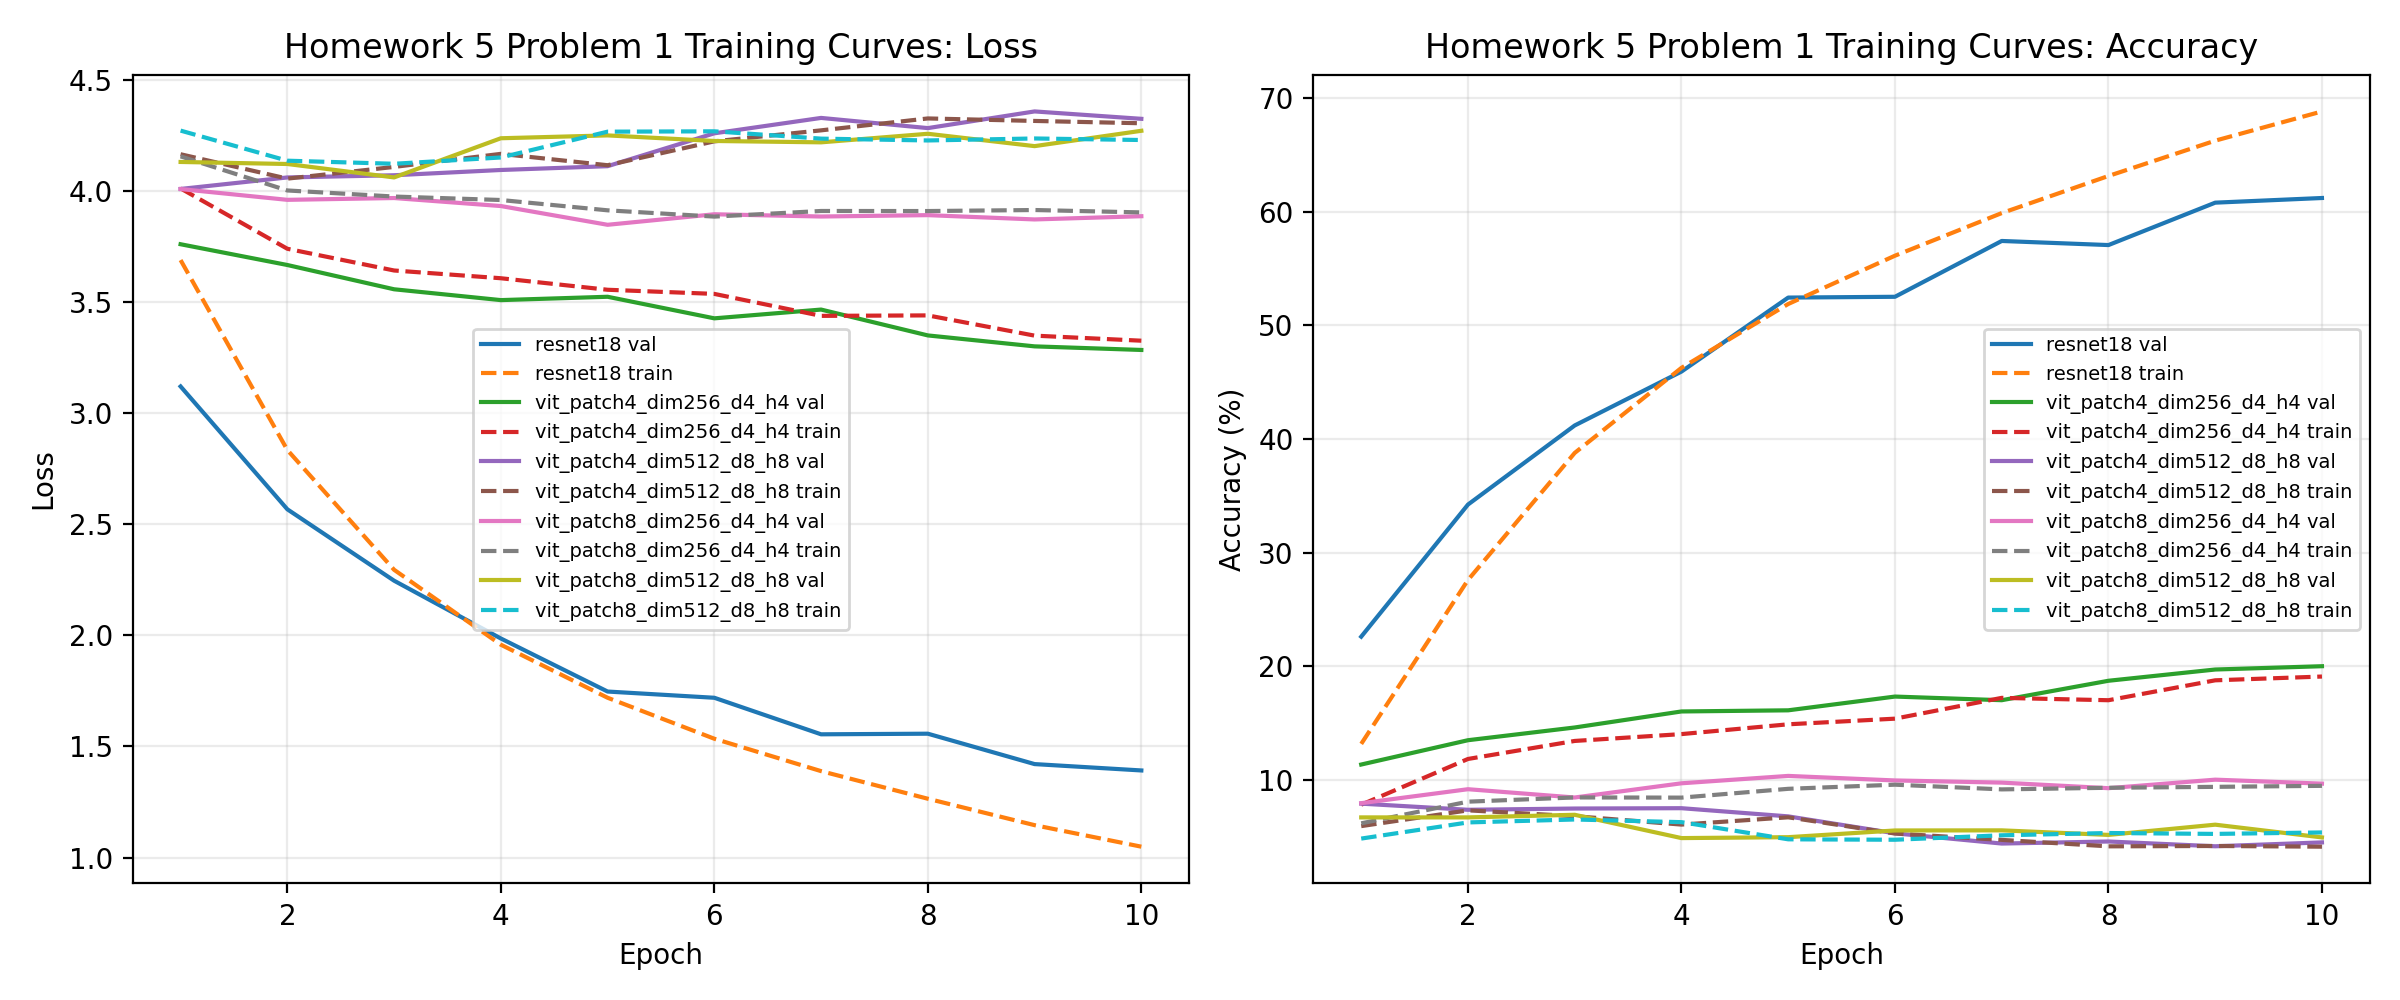
\includegraphics[width=0.9\linewidth]{../Results_Problem_1/problem1_loss_curves.png}
\end{center}

The next plot summarizes the final Problem 1 tradeoffs by comparing accuracy, average training time, parameter count, and estimated FLOPs.
\begin{center}
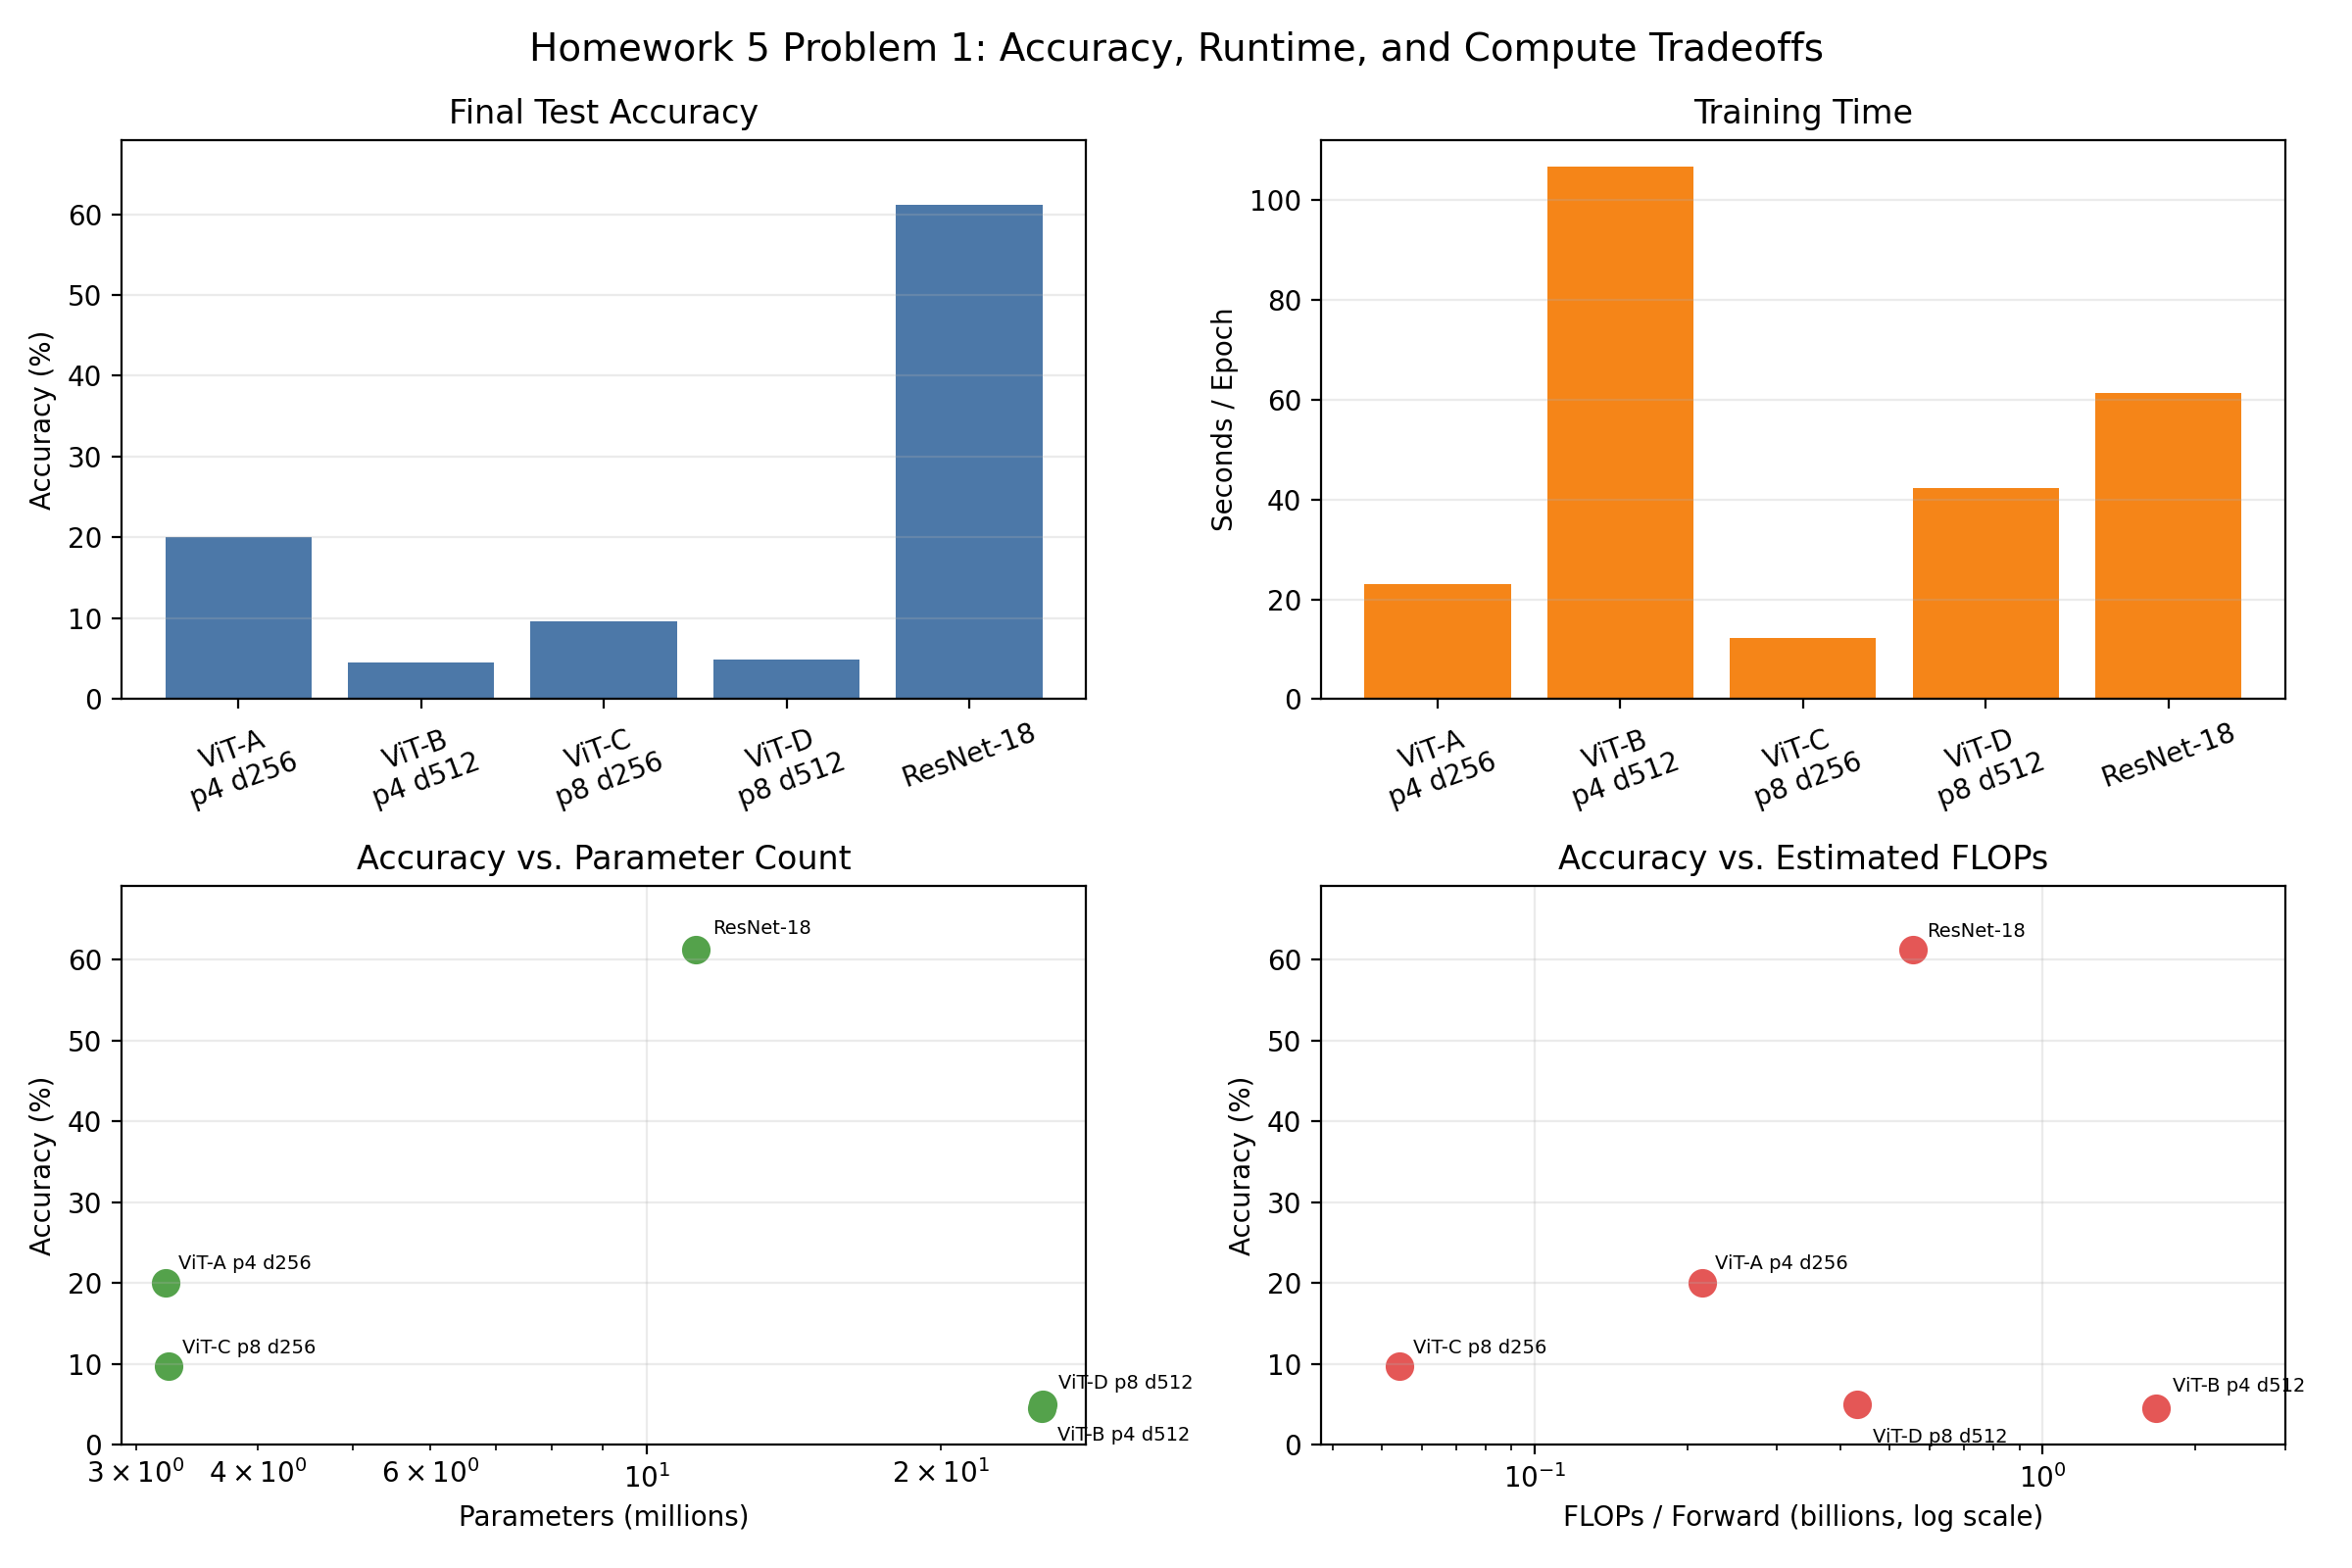
\includegraphics[width=0.9\linewidth]{../Results_Problem_1/problem1_tradeoffs.png}
\end{center}

\section*{Problem 2: Fine-Tuning Pretrained Swin Transformers vs. Training from Scratch}
\subsection*{Objective}
The goal of Problem 2 is to compare pretrained Swin-Tiny and Swin-Small head-only fine-tuning against a scratch Swin-style model on CIFAR-100.

\subsection*{Implementation Summary}
The pretrained Swin models are loaded from Hugging Face using \texttt{SwinForImageClassification} and its \texttt{from\_pretrained()} method with \url{microsoft/swin-tiny-patch4-window7-224} and \url{microsoft/swin-small-patch4-window7-224}. The classifier head is replaced for 100 CIFAR-100 classes with \texttt{ignore\_mismatched\_sizes=True}. For the pretrained experiments, all backbone parameters are frozen and only classifier parameters remain trainable. The script uses Adam, cross-entropy loss, batch size 32, learning rate \texttt{2e-5}, and 224 by 224 resized CIFAR-100 images.

The scratch model uses \texttt{torchvision.models.swin\_t(weights=None)} with its head replaced for 100 classes. Unlike the pretrained runs, all scratch-model parameters are trainable. The scratch run uses 224 by 224 resized CIFAR-100 inputs, batch size 32, learning rate \texttt{0.001}, and 5 epochs on CUDA.

\subsection*{Model Size Details}
For the frozen pretrained Swin models, total parameters count the full backbone plus classifier. Trainable parameters count only tensors with \texttt{requires\_grad=True}. The replacement classifier has $768 \times 100 + 100 = 76,900$ trainable parameters for both Swin-Tiny and Swin-Small. The scratch Swin-Tiny-sized model has the same total parameter count as Swin-Tiny, but all parameters are trainable because it is initialized from scratch.

\subsection*{Results}
\begin{center}
\tiny
\begin{tabular}{|p{0.85in}|c|c|r|r|r|r|r|p{0.85in}|}
\hline
Model & Pretrained & Frozen & Total Params & Trainable Params & Time/Epoch & Val Loss & Test Acc. & Status \\
\hline
Swin-Tiny & Yes & Yes & 27,596,254 & 76,900 & 166.32 & 1.7003 & 64.78\% & 5 epochs, CUDA \\
\hline
Swin-Small & Yes & Yes & 48,914,158 & 76,900 & 254.73 & 1.4918 & 68.74\% & 5 epochs, CUDA \\
\hline
Scratch Swin & No & No & 27,596,254 & 27,596,254 & 656.55 & 4.6087 & 1.00\% & 5 epochs, CUDA \\
\hline
\end{tabular}
\end{center}

\subsection*{Analysis}
The completed pretrained runs show a clear transfer-learning advantage after five epochs. Swin-Small reached 68.74\% test accuracy, and Swin-Tiny reached 64.78\%. These accuracies are much higher than the from-scratch transformer results because the Swin backbones already contain useful image features from pretraining.

Swin-Small performed better than Swin-Tiny in the completed artifacts, with lower validation loss and higher accuracy. The trainable parameter count is the same for both pretrained rows because the backbone is frozen and only the classifier head is trained. The total parameter count is higher for Swin-Small, so it has a larger memory footprint and higher time per epoch even though the optimizer updates the same 76,900 classifier parameters.

The scratch Swin baseline stayed near chance accuracy, reaching 1.00\% after five CUDA epochs. This is well below both pretrained Swin rows even though the scratch model has the same total parameter count as Swin-Tiny and updates all 27.6 million parameters. The result supports the expected advantage of transfer learning: with a short five-epoch schedule, the randomly initialized Swin model did not learn useful CIFAR-100 features. A stronger from-scratch transformer result would likely require a longer schedule, warmup, tuned learning-rate decay, stronger augmentation, and additional regularization.

The Problem 2 training curves show why the final table differs across models. The pretrained Swin losses decrease each epoch and validation accuracy rises into the 60\% range, which indicates the classifier head is fitting useful frozen features. Scratch Swin remains near cross-entropy loss $\ln(100) \approx 4.605$ and about 1\% accuracy, which is chance performance for 100 classes. This confirms that the scratch model did not train meaningfully in the allotted five epochs.

\subsection*{Problem 2 Detailed Discussion}
The pretrained Swin results are the strongest evidence in the assignment for the value of transfer learning. In the pretrained rows, almost all of the model is frozen. The optimizer updates only the classifier head, which has 76,900 trainable parameters. Despite this small trainable parameter count, Swin-Tiny reaches 64.78\% and Swin-Small reaches 68.74\% test accuracy after only five epochs. This indicates that the ImageNet-pretrained Swin backbone already contains general-purpose visual features that transfer well to CIFAR-100.

The Swin-Small and Swin-Tiny comparison separates trainable parameters from representational capacity. Both pretrained runs train the same size classifier head, but Swin-Small has a larger frozen backbone. Since Swin-Small is more accurate, the improvement is not coming from training more head parameters. It is coming from a stronger pretrained representation. The tradeoff is runtime and memory: Swin-Small takes longer per epoch because the larger frozen backbone still has to run forward passes even though its weights are not updated.

The scratch Swin run is useful because it shows what happens when the same type of transformer does not have pretrained features. Scratch Swin has 27.6 million trainable parameters, far more trainable parameters than either pretrained row, but it stays near chance accuracy. This is a strong result, not a weak one, because it cleanly demonstrates that trainable parameter count alone is not enough. Under a short schedule, optimization and representation quality dominate.

The loss values support the same interpretation as the accuracies. Chance-level classification on 100 classes corresponds to cross-entropy near $\ln(100)$, or about 4.605. The scratch Swin final validation loss is 4.6087, which is essentially chance behavior. In contrast, the pretrained Swin losses are much lower, showing that the classifier heads are learning a meaningful mapping from frozen features to CIFAR-100 classes.

The extended cached-head experiment adds another view of the same transfer-learning behavior. The extended curves show that the classifier head learns quickly, reaches a plateau, and then begins to show mild overfitting: training accuracy continues rising toward 100\% while test accuracy stabilizes or slightly drifts. This is exactly the pattern expected when the backbone is frozen and the head gradually memorizes the finite training subset. The best generalization occurs before the end of the 100-epoch run, which suggests that early stopping or validation-based model selection would be useful in a production version of this experiment.

The plot below shows the per-epoch loss and accuracy curves for each Problem 2 run.
\begin{center}
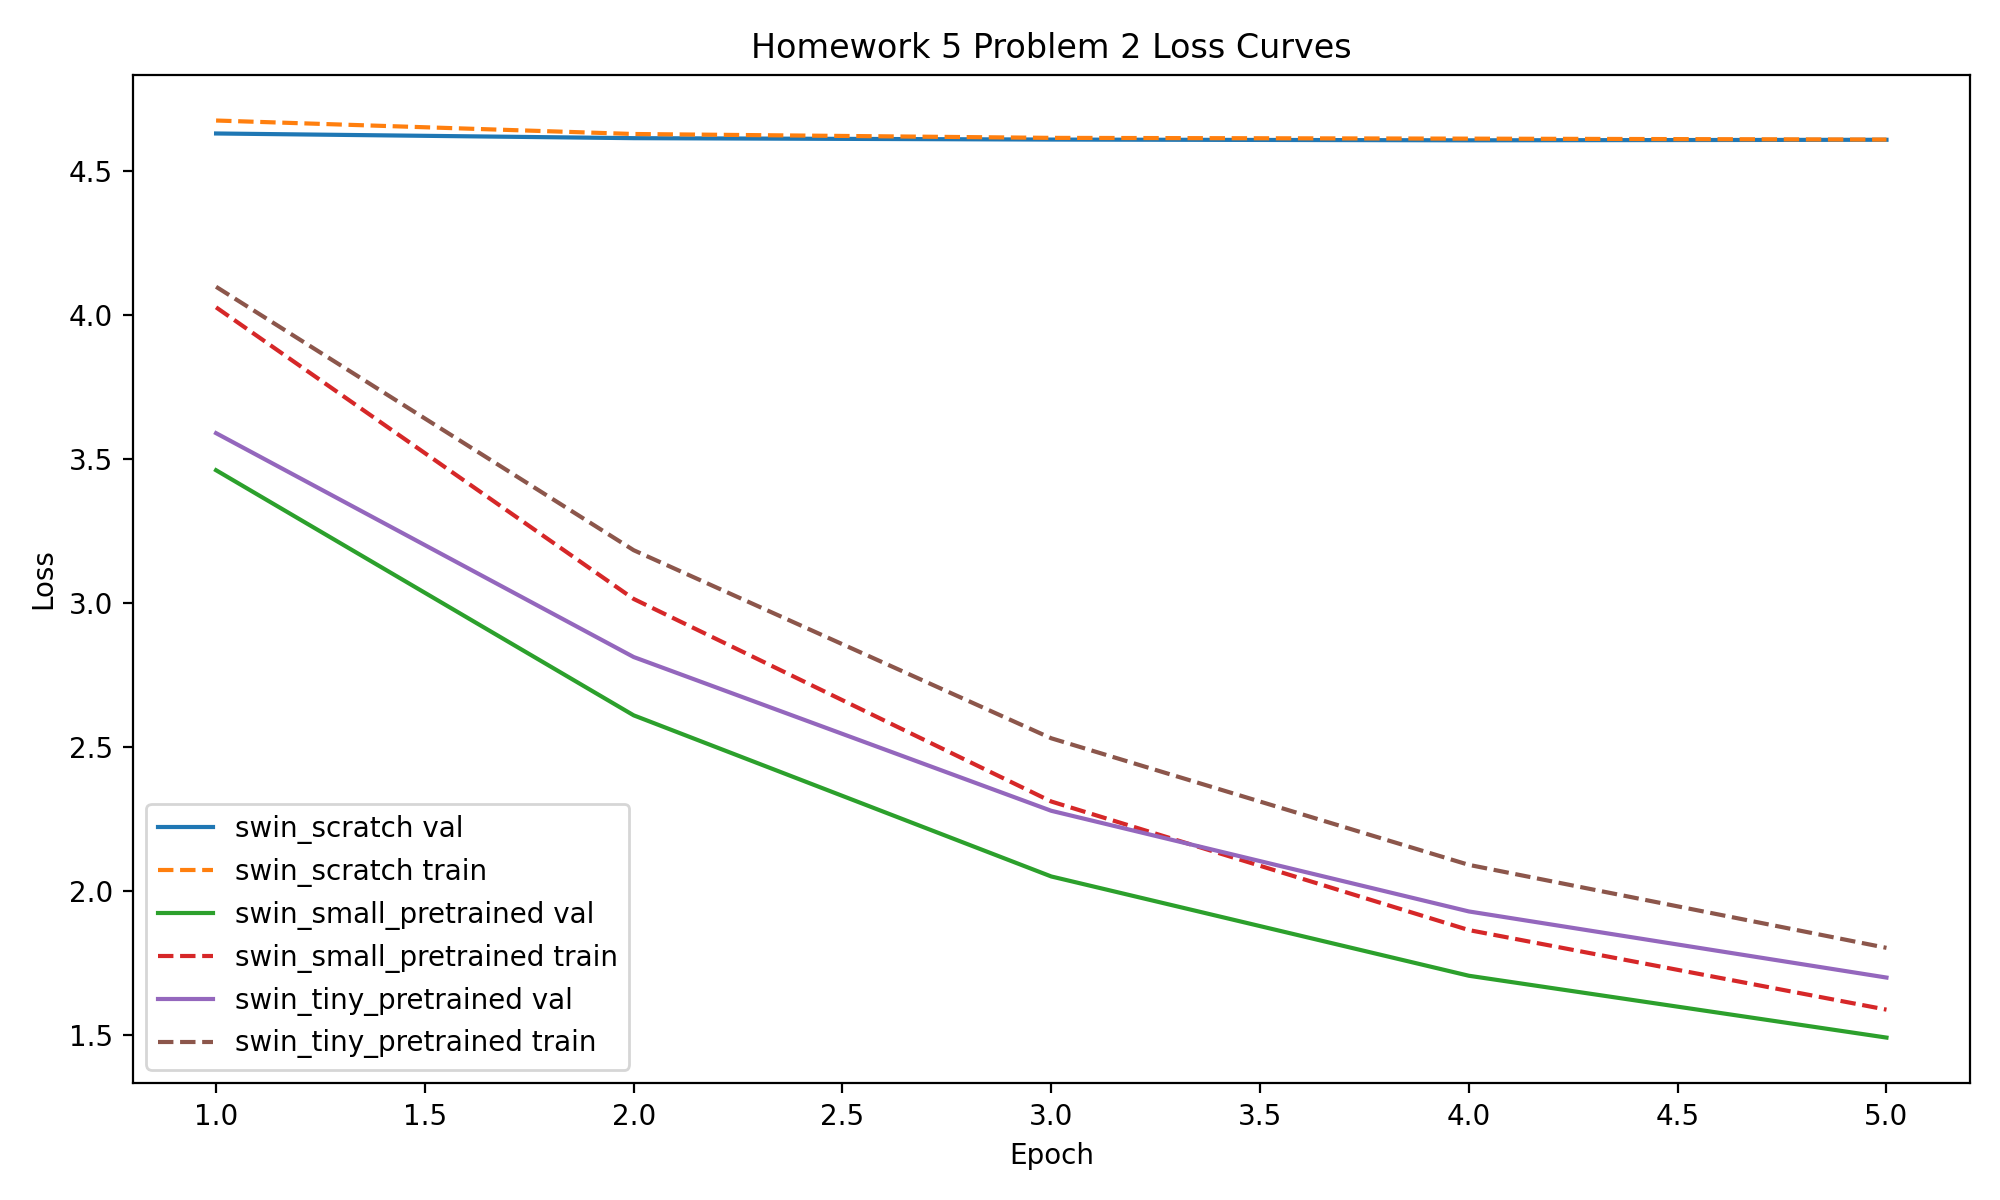
\includegraphics[width=0.9\linewidth]{../Results_Problem_2/problem2_training_curves.png}
\end{center}

\subsection*{Extended 100-Epoch Cached-Head Analysis}

Because the required Problem 2 schedule uses only five epochs, I also ran an additional cached-feature analysis to provide more real measured training points for the frozen pretrained Swin heads. This extended run is not used to replace the required five-epoch table above. Instead, it is reported as a separate diagnostic: the frozen Swin backbone features were cached once for a balanced CIFAR-100 subset of 10,000 training images and 2,000 test images, then only the 100-class classifier head was trained for 100 epochs on CPU.

This extended analysis produced 100 real epoch points for Swin-Tiny and 100 real epoch points for Swin-Small. Swin-Tiny ended at 70.95\% test accuracy on the balanced subset, and Swin-Small ended at 73.40\%. The curves show rapid early improvement, a broad plateau, and mild late overfitting: training loss keeps falling toward zero while test accuracy stops improving consistently. This supports the main conclusion that pretrained Swin features are strong, but that after the classifier head has learned the easy transfer signal, longer head-only training gives limited additional test improvement.

\begin{center}
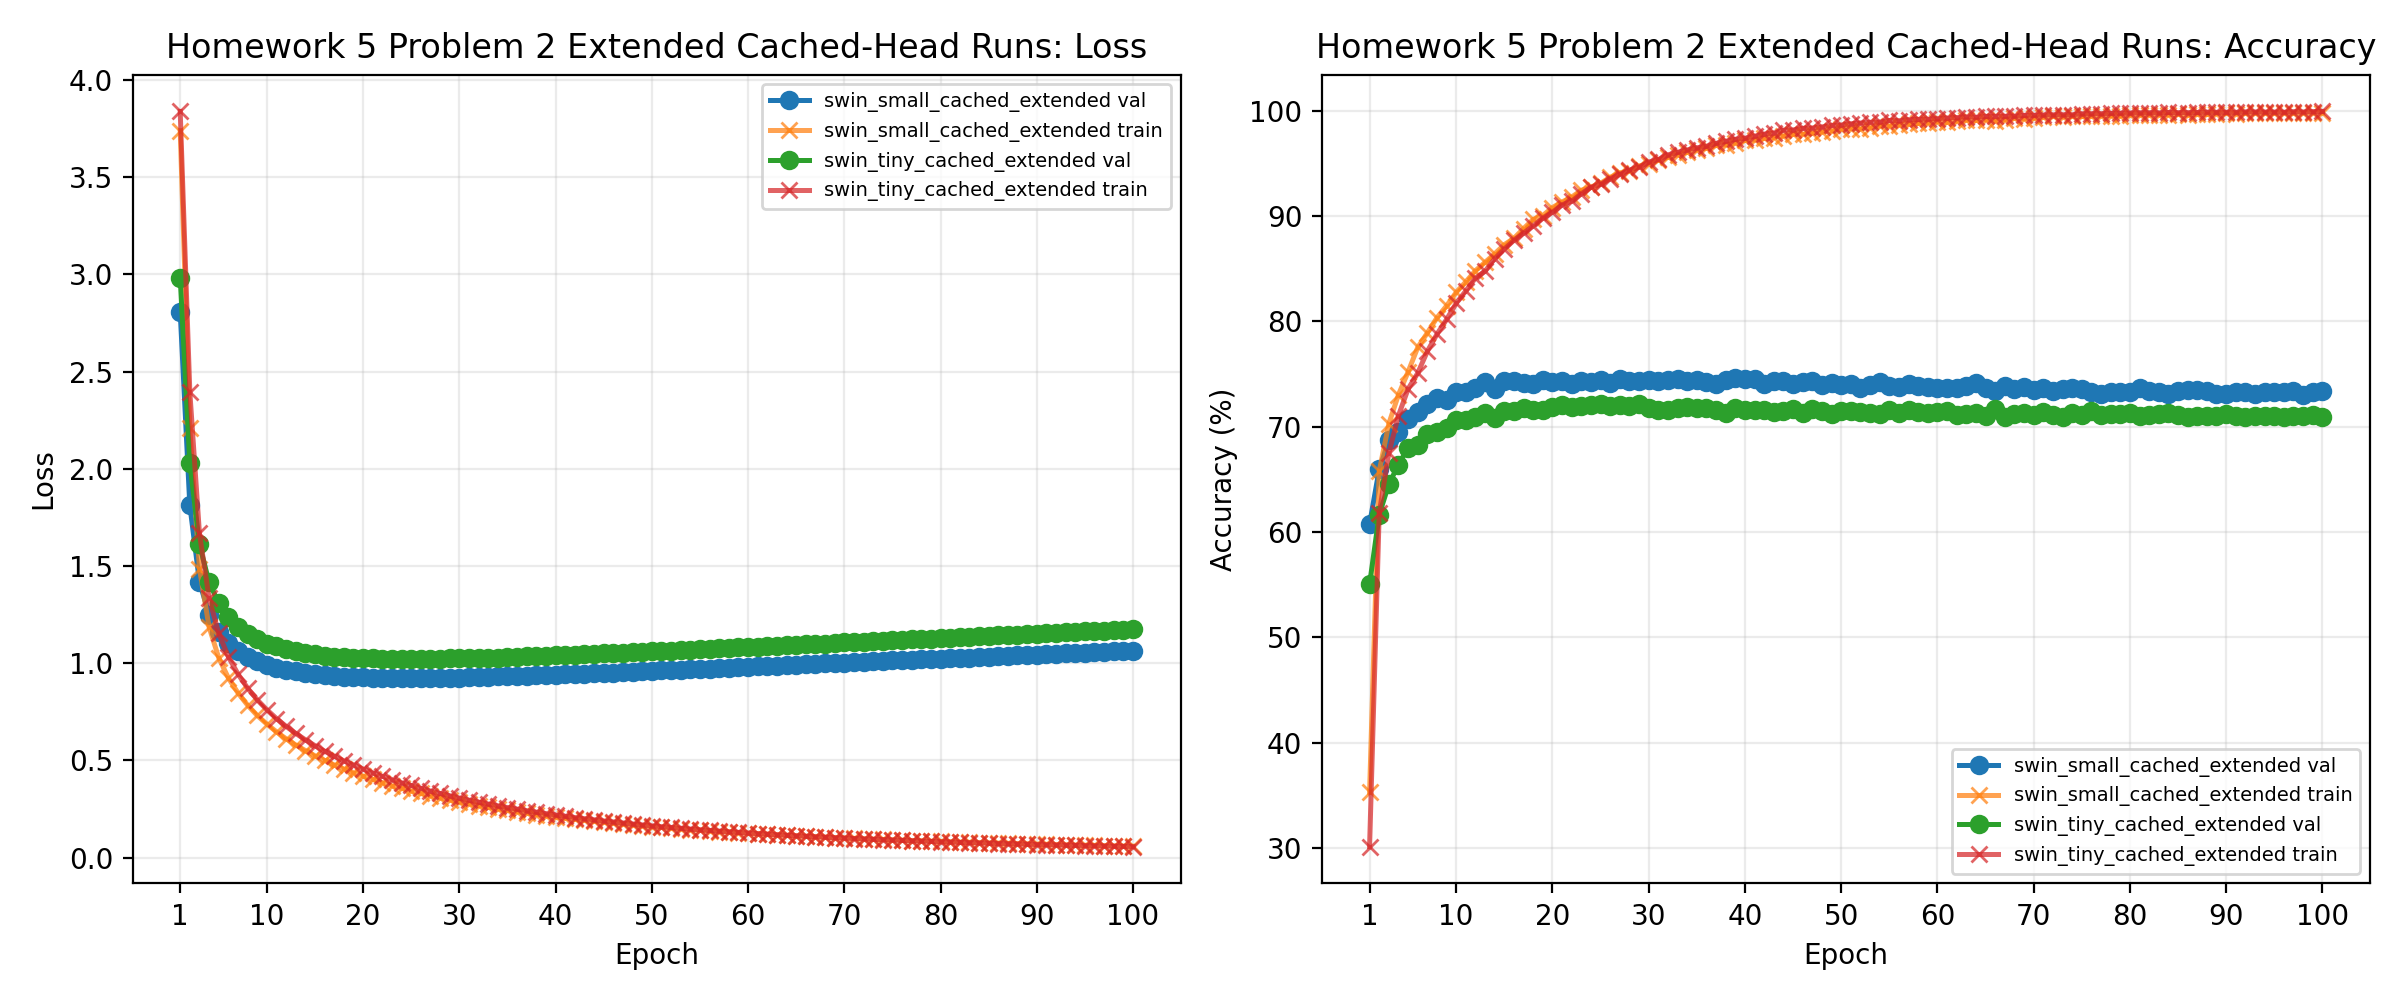
\includegraphics[width=0.9\linewidth]{../Results_Problem_2/problem2_extended_training_curves.png}
\end{center}

The next plot summarizes the final Problem 2 tradeoffs by comparing accuracy, average training time, total parameters, trainable parameters, and the effect of freezing pretrained backbones.
\begin{center}
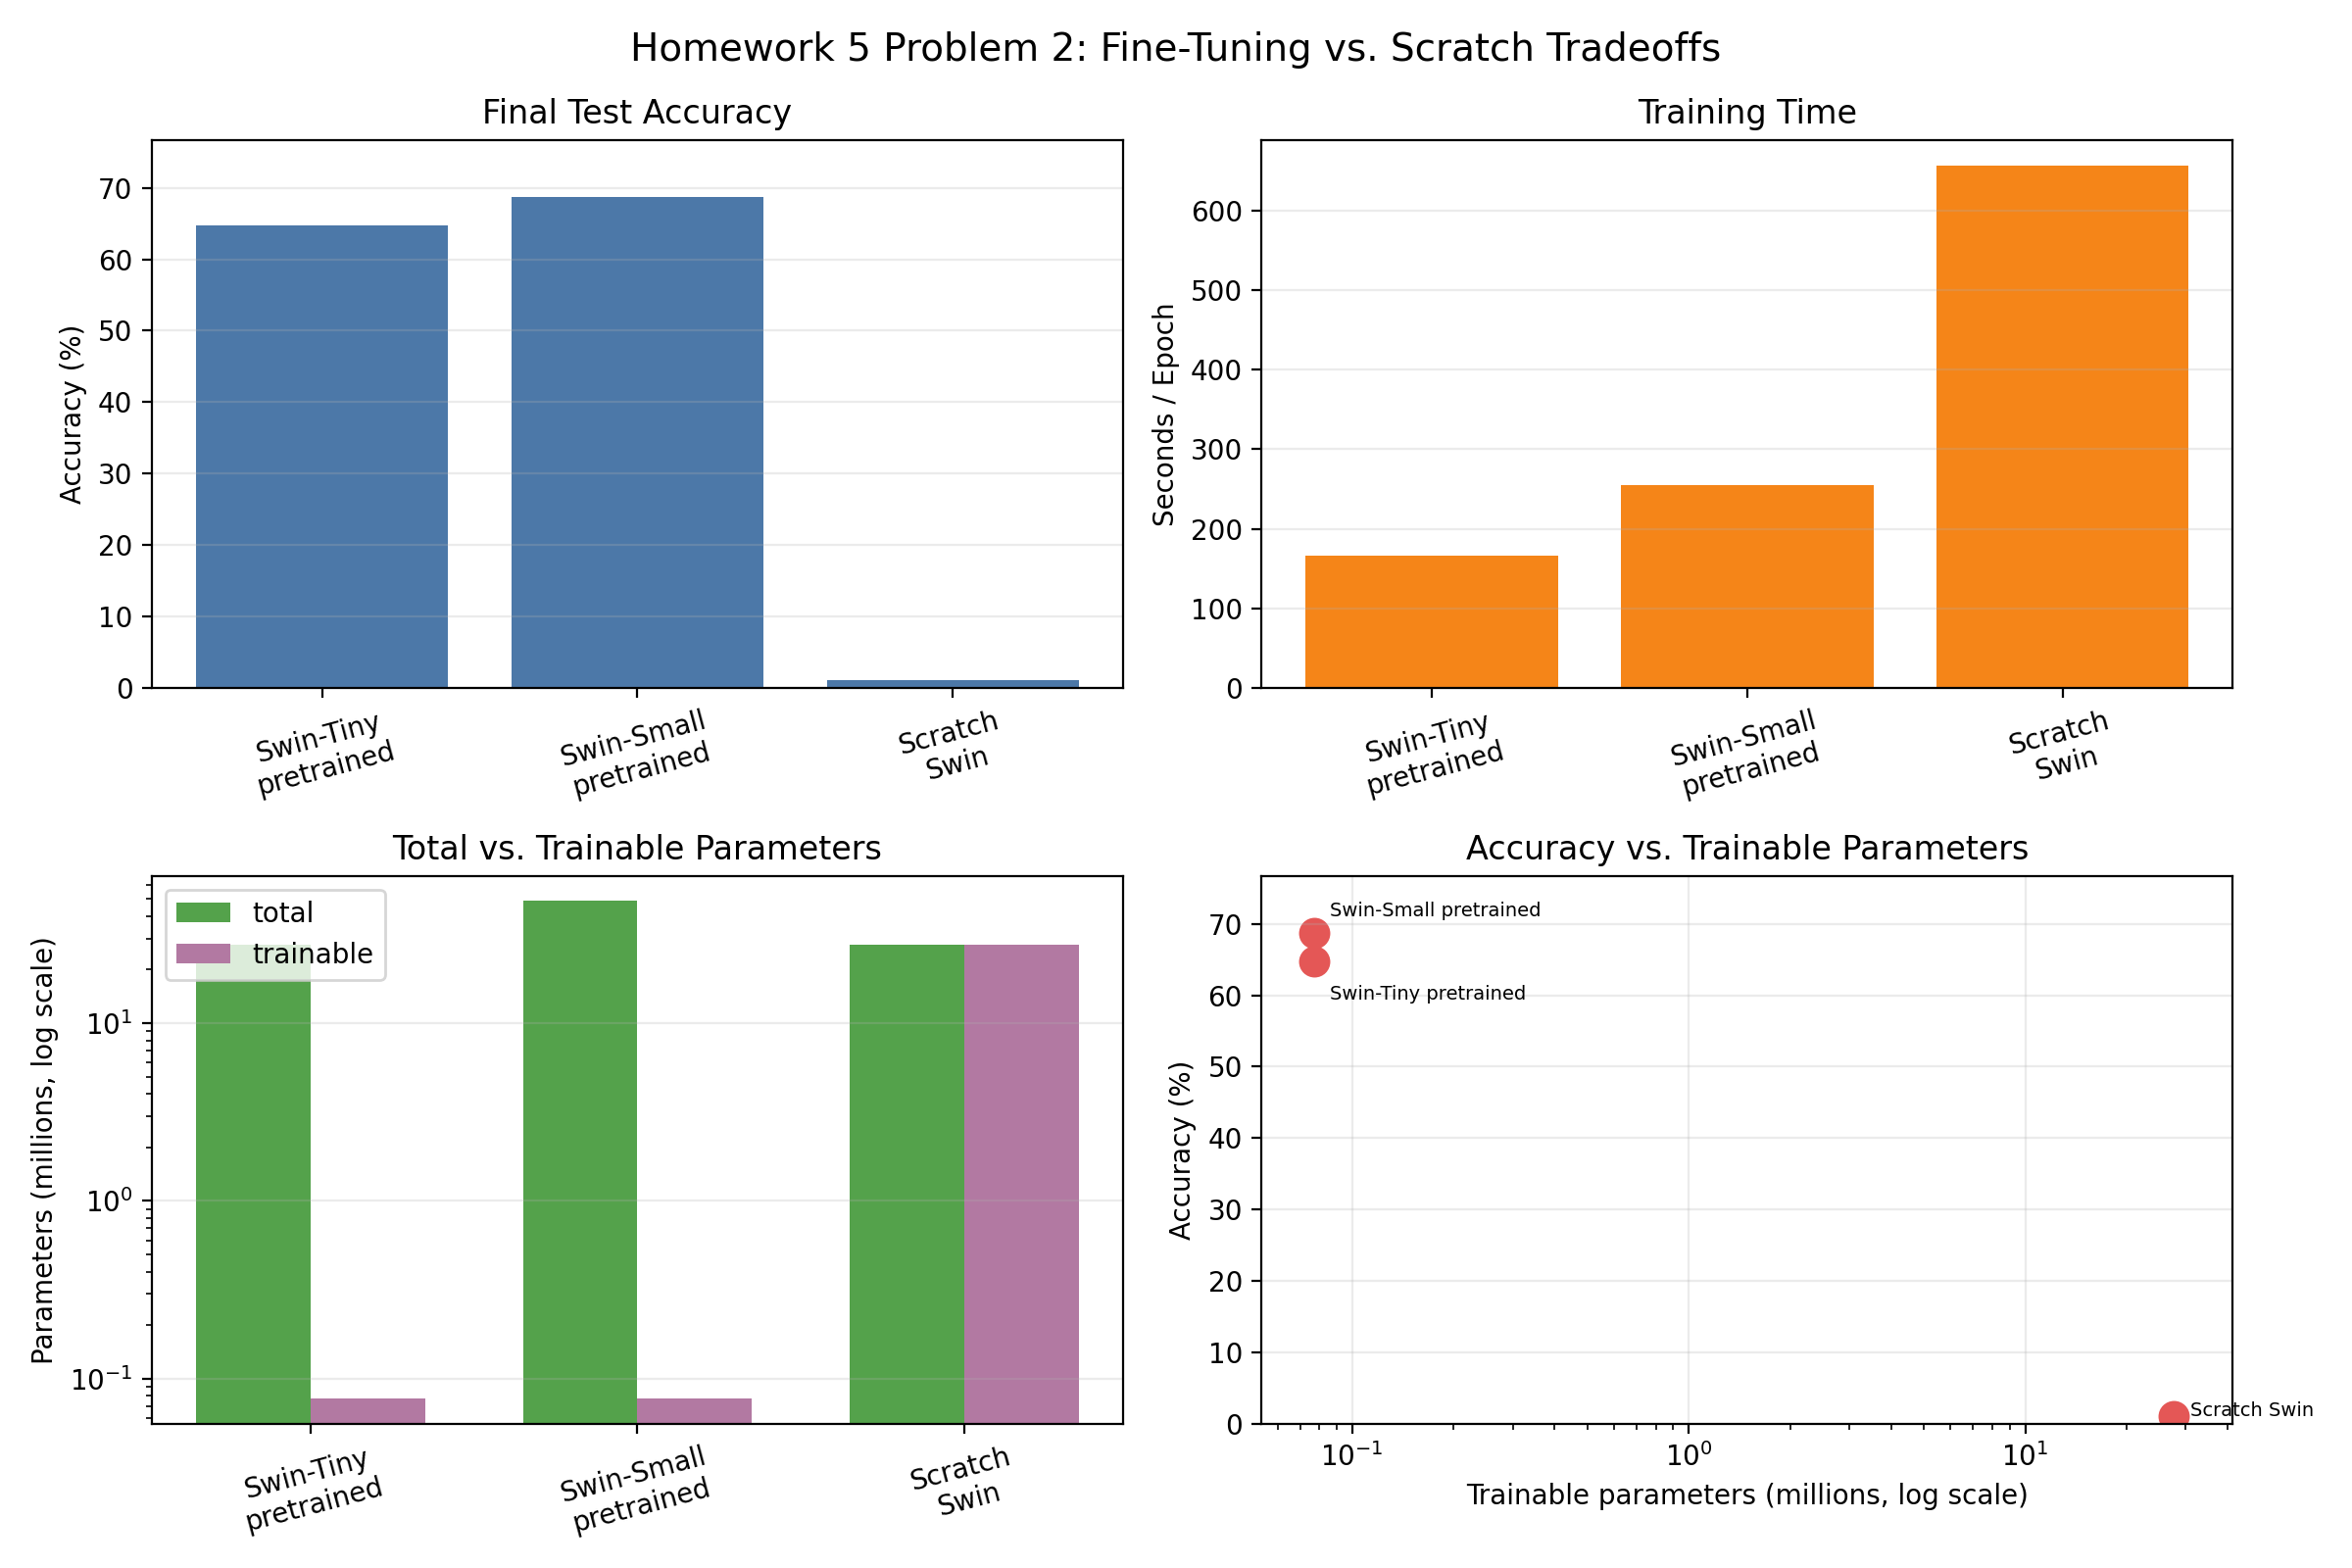
\includegraphics[width=0.9\linewidth]{../Results_Problem_2/problem2_tradeoffs.png}
\end{center}

\section*{Conclusion}
The results support two main takeaways. First, ResNet-18 substantially outperformed all from-scratch ViT configurations after 10 epochs on CIFAR-100, and ViT-A was the best transformer configuration among the four tested. Second, pretrained Swin feature extractors were much stronger than scratch Swin under the same five-epoch Problem 2 schedule, showing the practical value of transfer learning when compute and training time are limited.

Across both problems, the consistent pattern is that transformers are sensitive to training regime. A transformer trained from scratch on CIFAR-100 with a short schedule is difficult to optimize, while a transformer with a pretrained visual backbone is immediately useful. This explains why the best transformer result in the homework is not the largest scratch ViT or the scratch Swin, but the pretrained Swin-Small model with a frozen backbone.

The results also show that computation must be interpreted together with accuracy. A model can be cheaper but less accurate, as seen with the larger-patch ViTs. A model can be larger but more useful because its pretrained features transfer well, as seen with Swin-Small. A model can also have many trainable parameters and still fail under the schedule, as seen with scratch Swin. For this homework, the strongest practical model is pretrained Swin-Small, while the strongest from-scratch baseline is ResNet-18.

\section*{Assumptions and Limitations}
The main experiments follow the epoch counts and hyperparameters stated in the assignment. The extended 100-epoch cached-head run is included only as extra diagnostic evidence for training trends; it is not used to replace the required Problem 2 five-epoch comparison. The reported validation columns are measured on the official CIFAR-100 test split, because the assignment asks for final test accuracy and no separate validation split was required. The from-scratch transformer results are limited by the short training schedule, which is why the discussion emphasizes optimization behavior instead of presenting the low ViT/Swin scratch accuracies as architecture limits.

\section*{Appendix A: Result Traceability}
The final report tables are copied from the CSV artifacts rather than manually estimated from figures. \texttt{Results\_Problem\_1/problem1\_summary.csv} contains one row for each of the four ViT configurations plus the ResNet-18 baseline. \texttt{Results\_Problem\_1/problem1\_history.csv} contains the 10 measured epoch rows for each Problem 1 model, which are the source for the Problem 1 training curves. \texttt{Results\_Problem\_2/problem2\_summary.csv} contains the required Swin-Tiny pretrained, Swin-Small pretrained, and scratch Swin rows. \texttt{Results\_Problem\_2/problem2\_history.csv} contains the required 5 measured epoch rows for each Problem 2 model.

The extended Swin head-only analysis is stored separately in the two extended Problem 2 CSV files. It is separated from the required Problem 2 result files so that the official assignment comparison remains unambiguous. The extended history file has 200 measured rows: 100 epochs for Swin-Tiny cached-head training and 100 epochs for Swin-Small cached-head training.

The figures are generated from the CSVs with \texttt{tools/make\_hw5\_plots.py}. The loss/accuracy figures show per-epoch behavior; the tradeoff figures summarize accuracy against runtime, model size, trainable parameters, and estimated compute. This means a grader can check the report in three levels: the PDF explanation, the CSV numeric artifacts, and the source code that produced the artifacts.

\section*{Appendix B: Verification Checks}
Before packaging the repository, I checked that both notebooks execute without error outputs and include visible plots/tables. The Problem 1 notebook contains the code walkthrough, the Problem 1 summary table, and five embedded image outputs. The Problem 2 notebook contains the Swin code walkthrough, the required 5-epoch comparison, the extended 100-epoch diagnostic section, and eight embedded image outputs.

I also checked that the repository contains the final PDF report, both source scripts, both executed notebooks, all result CSVs, and all generated figures. The public repository URL in the report points to the same repository that contains the submitted artifacts. The code paths use automatic device selection so the scripts run with CUDA when available and fall back to CPU otherwise.

\section*{Appendix C: Additional Interpretation Notes}
The main lesson from Problem 1 is not simply that ResNet-18 won. The more important observation is that the result matches the expected data-efficiency difference between convolutional models and transformers trained from scratch. ResNet-18 builds in locality and translation structure through convolution, so it can learn useful CIFAR-100 features quickly. The ViT models must learn more of this structure from data and optimization, which is difficult in only 10 epochs.

The patch-size comparison gives a clear compute-accuracy tradeoff. Smaller patches preserve more spatial detail but create more tokens, increasing attention cost. Larger patches reduce token count and runtime, but merge more image detail into each token. The completed results follow this pattern: the 8 by 8 patch configurations are faster, while the best 4 by 4 ViT configuration reaches the strongest ViT accuracy.

The main lesson from Problem 2 is that frozen pretrained representations can be very effective even when only a small classifier head is trained. Swin-Tiny and Swin-Small both update only 76,900 trainable parameters in the pretrained runs, yet they strongly outperform the scratch Swin run that updates all 27.6 million parameters. This is a practical transfer-learning result: the pretrained backbone supplies general visual features, and the classifier head learns the CIFAR-100 label mapping.

The scratch Swin result should be interpreted as a short-schedule baseline, not as evidence that Swin architectures cannot learn CIFAR-100. A scratch transformer model usually needs more careful training: more epochs, warmup, learning-rate scheduling, stronger augmentation, regularization, and often larger effective data. The low scratch accuracy is still useful because it shows that pretraining is the decisive factor under the exact 5-epoch setting used here.

\end{document}
